% CAPITULO 2-------------------------------------------------------------------

\chapter{TAREFA 2: SISTEMAS DISTRIBUÍDOS}
\label{sec:tarefa2}

Os sistemas distribuídos são peças de software usadas para coordenar as ações de vários computadores. Essa coordenação é alcançada através da troca de mensagens, isto é, com pedaços de dados que transmitem informações.

Os sistemas distribuídos requerem componentes simultâneos, uma rede de comunicação e um mecanismo de sincronização. Eles permitem que recursos, incluindo software, sejam compartilhados por sistemas conectados a uma rede. Portanto, o sistema é baseado em uma rede que conecta computadores e lida com o roteamento de mensagens.

A computação distribuída é uma área da computação responsável pela análise de sistemas distribuídos. O programa de computador executado em um sistema distribuído é chamado de programa distribuído.

Em um contexto no qual pode haver centenas ou milhares de computadores, o que é uma proporção comum em grandes empresas de Internet, é muito comum que haja falhas de componentes, sejam elas hardware, rede, discos, etc., e o sistema deve ser preparado para enfrentá-los em todos os momentos.

\section{Distribuição de Dados}
\label{distribuicao}

A distribuição é essencial para lidar com \textit{clusters} de dados muito grandes. É necessário obter escalabilidade, que é o meio de manter um desempenho estável quando os conjuntos de dados crescem adicionando novos recursos ao sistema.

Por outro lado, a distribuição apresenta uma série de problemas técnicos que tornam importante o design e a implementação de armazenamento e computação distribuídos. Um ponto a ser levado em consideração é o risco de possíveis falhas.


\section{Características dos sistemas distribuídos}
\label{caracteristica}

\textbf{Compatibilidade}

Os dispositivos podem funcionar com diferentes sistemas operacionais. Isso não os impede de oferecer sempre os mesmos serviços aos usuários. Por esse motivo, todos os dispositivos conectados são compatíveis entre si.

Outra questão fundamental é o design do software, porque também é compatível com todos os sistemas e usuários que estão em cada computador.

\textbf{Tolerância ao erro}

Sendo uma rede única com muitos computadores, se algum de seus componentes falhar, os outros poderão continuar executando sua função completamente, evitando erros rapidamente.

Por esse motivo, os sistemas distribuídos tendem a fornecer muita confiança ao trabalhar com eles, porque é muito raro o sistema falhar completamente, porque as tarefas não residem em um único dispositivo, mas em computadores diferentes.

\textbf{Middleware e API}

Processadores diferentes usam \textit{middleware} de distribuição, ajudando a compartilhar diferentes recursos e capacidades para fornecer aos usuários uma rede consistente e integrada. Ele também oferece aos aplicativos diversos serviços, como segurança e recuperação de falhas.

Atualmente, mais se ouve sobre APIs (interfaces de programação de aplicativos), que funcionam como um \textit{gateway} através do qual os aplicativos podem se comunicar. Os aplicativos não precisam saber nada sobre outros aplicativos, exceto sua API.

\begin{figure}[H]
    \centering
    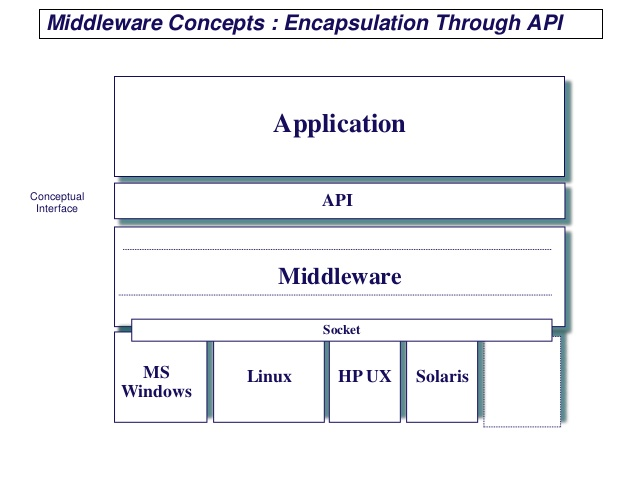
\includegraphics[width=0.7\linewidth]{dados/figuras/middleware}
    \caption{Middleware}
    \label{fig:middleware}
\end{figure}

Exemplos comuns de \textit{middleware} incluem \textit{middleware} de banco de dados, \textit{middleware} de servidor de aplicativos, \textit{middleware} orientado a mensagens, \textit{middleware} de web e monitores de processamento de transações. Normalmente, cada programa oferece serviços de sistemas de mensagens para que diversos aplicativos possam se comunicar utilizando estruturas de mensagens como protocolo SOAP, serviços Web, REST (representational state transfer) e JSON (JavaScript Object Notation).

Embora todos os tipos de \textit{middleware} executem funções de comunicação, o tipo que uma empresa escolherá depende de qual serviço está sendo utilizado e qual tipo de informação deve ser comunicado. Isso pode incluir autenticação de segurança, gerenciamento de transações, consultas de mensagens, servidores de aplicativos, servidores da web e diretórios. O \textit{middleware} também pode ser utilizado para processamento distribuído com ações que ocorrem em tempo real em vez de envio e recebimento repetitivo de dados.

\section{Arquitetura Sugerida}

Para a Empresa de Roupas T-Shirt, decidiu-se utilizar a arquitetura distribuída, por ela ser mais dinâmica, no permite otimizar todo o sistema da empresa. Abaixo citaremos algumas das vantagens em optar por esta arquitetura distribuída.

\begin{tabular}{@{$\bullet$ }ll}
	melhor relação custo/benefício; \\
	maior capacidade de processamento; maior domínio de aplicações; \\
	maior confiabilidade; \\
	maior disponibilidade; \\
	crescimento gradativo de sua capacidade de processamento.
\end{tabular}

